\documentclass[twoside]{article} 
\usepackage[utf8]{inputenc}
\usepackage{amsmath}
\usepackage{amsfonts}
\usepackage[pdftex]{graphicx}
\usepackage[procnames]{listings}
\usepackage{color}
\usepackage{lipsum} % Package to generate dummy text throughout this template
\usepackage{braket}
\usepackage{epsfig}
\usepackage{epstopdf}


% \usepackage[sc]{mathpazo} % Use the Palatino font
\usepackage[T1]{fontenc} % Use 8-bit encoding that has 256 glyphs
% \linespread{1.05} % Line spacing - Palatino needs more space between lines
% \usepackage{microtype} % Slightly tweak font spacing for aesthetics

\usepackage[hmarginratio=1:1,top=32mm,columnsep=20pt]{geometry} % Document margins
\usepackage{multicol} % Used for the two-column layout of the document
\usepackage[width=.8\textwidth,hang, small,labelfont=bf,up,textfont=it,up]{caption} % Custom captions under/above floats in tables or figures
\usepackage{float} % Required for tables and figures in the multi-column environment - they need to be placed in specific locations with the [H] (e.g. \begin{table}[H])
\usepackage{hyperref} % For hyperlinks in the PDF

\usepackage{lettrine} % The lettrine is the first enlarged letter at the beginning of the text
\usepackage{paralist} % Used for the compactitem environment which makes bullet points with less space between them
\usepackage{todonotes}
\newcommand{\unit}[1]{\ensuremath{\; \mathrm{#1}}}

\usepackage[super]{nth}
\usepackage{bm}
\usepackage[version=4]{mhchem}
\usepackage[inline]{enumitem}

\usepackage{abstract} % Allows abstract customization
\renewcommand{\abstractnamefont}{\normalfont\bfseries} % Set the "Abstract" text to bold
\renewcommand{\abstracttextfont}{\normalfont\small\itshape} % Set the abstract itself to small italic text

\usepackage{titlesec} % Allows customization of titles

\usepackage{fancyhdr} % Headers and footers

\usepackage[labelformat=simple]{subcaption}
\renewcommand\thesubfigure{(\alph{subfigure})}

\newcommand{\spfield}{\mathcal{E}_\ell^{(1)}}
\newcommand{\sprabi}{\Omega_1^{(1)}}
\newcommand{\me}{\mathrm{e}}
\usepackage{siunitx}
\sisetup{
	separate-uncertainty = true,
	multi-part-units = single
}

\DeclareSIUnit{\belm}{Bm}
\DeclareSIUnit{\gauss}{G}

\newcommand{\qop}[1]{\hat{#1}}
\newcommand{\qproj}[1]{\ket{#1}\bra{#1}}
\newcommand{\device}[1]{\textit{#1}}
\newcommand{\expval}[1]{\left\langle #1 \right\rangle}
\newcommand{\subcapref}[1]{\subcap{\subref{#1}}}
\newcommand{\subcap}[1]{\textbf{#1}~|}
\newcommand{\realpart}{\operatorname{Re}}

\newcommand{\matr}[1]{\bm{#1}}
\newcommand{\sx}{\matr{\sigma}_x}
\newcommand{\sy}{\matr{\sigma}_y}
\newcommand{\sz}{\matr{\sigma}_z}
\newcommand{\eff}{\text{eff}}
\newcommand{\real}{\text{real}}

\DeclareCaptionLabelSeparator{pipe}{ | }

\captionsetup{% use subfigure to confine changes to subcaptions
  font={sf},
  textfont={up},
  labelsep=pipe,
  format=plain,
  width=\textwidth
}

\captionsetup[subfigure]{
	format=hang,
	labelsep=pipe
}

\usepackage[backend=biber, sorting=none, style=nature]{biblatex}
\DeclareNameAlias{sortname}{given-family}
\DeclareNameAlias{default}{given-family}
\bibliography{master}

\setlength{\marginparwidth}{3cm}

\renewcommand\thesection{\arabic{section}} % Roman numerals for the sections
\renewcommand\thesubsection{\thesection.\arabic{subsection}} % Roman numerals for subsections
\titleformat{\section}[block]{\large\scshape\centering}{\thesection.}{1em}{} % Change the look of the section titles
\titleformat{\subsection}[block]{\large}{\thesubsection.}{1em}{} % Change the look of the section titles


\pagestyle{fancy} % All pages have headers and footers
\fancyhf{}
\fancyhead[C]{Notes on project in DiVincenzo group $\bullet$ 2017} % Custom header text
\fancyfoot[RO,LE]{\thepage} % Custom footer text
\fancyfoot[CO,CE]{Jesse Slim}
\fancypagestyle{firststyle}
{	
	\fancyhf{}
	\renewcommand{\headrulewidth}{0pt}
	\fancyfoot[RO,LE]{\thepage}
	\fancyfoot[CO,CE]{Jesse Slim}
}


%----------------------------------------------------------------------------------------
%	TITLE SECTION
%----------------------------------------------------------------------------------------

\title{\vspace{-15mm}
	\fontsize{12pt}{10pt}\selectfont Research internship \\[1em]
	\fontsize{18pt}{10pt}\selectfont \textbf{Notes on project in DiVincenzo group}
} % Article title

\author{
	\large
	\textsc{Jesse Slim}\\ % Your name
}
\date{\normalsize\today\vspace{-8mm}}

%----------------------------------------------------------------------------------------


\begin{document}

\definecolor{keywords}{RGB}{255,0,90}
\definecolor{comments}{RGB}{0,0,113}
\definecolor{red}{RGB}{160,0,0}
\definecolor{green}{RGB}{0,150,0}

\lstset{language=Python, 
	basicstyle=\ttfamily\small, 
	keywordstyle=\color{keywords},
	commentstyle=\color{comments},
	stringstyle=\color{red},
	showstringspaces=false,
	identifierstyle=\color{green},
	procnamekeys={def,class}}

\maketitle % Insert title
\thispagestyle{firststyle} % Only footer on first page

%----------------------------------------------------------------------------------------
%	ABSTRACT
%----------------------------------------------------------------------------------------

\vspace{1em}
\begin{abstract}
\noindent  
Magnus expansion
	
\end{abstract}
\newpage

\tableofcontents





%----------------------------------------------------------------------------------------
%	ARTICLE CONTENTS
%----------------------------------------------------------------------------------------
\newpage
\section{The truncated Magnus expansion}
The Magnus expansion\supercite{Magnusexponentialsolutiondifferential1954,WaughAverageHamiltonianTheory2007,BlanesMagnusexpansionits2009,BlanespedagogicalapproachMagnus2010} for the time evolution under Hamiltonian $H(t)$ is defined as
\begin{alignat}{2}
	&\Omega(t,t_0) &&= \sum_{n=1}^\infty \Omega_n(t,t_0),\\
	&\Omega_1(t,t_0) &&= \int_{t_0}^t \mathrm{d}t_1 \tilde{H}(t_1),\label{eq:omg-1}\\
	&\Omega_2(t,t_0) &&= -\frac{1}{2}\int_{t_0}^t \mathrm{d}t_1 \left[ \Omega_1(t_1,t_0), \tilde{H}(t_1) \right] = \frac{1}{2}\int_{t_0}^t \mathrm{d}t_1 \int_{t_0}^{t_1} \mathrm{d}t_2 \left[ \tilde{H}(t_1), \tilde{H}(t_2) \right] \label{eq:omg-2},
\end{alignat}
where $\tilde{H}(t) = -i / \hbar H(t)$. In the reminder of these notes, natural units with $\hbar = 1$ will be used.

We use this series to approximate the trajectory of a two-level qubit driven by an oscillating signal proportional to $\matr{\sigma}_x$ in the lab frame. To this end, we use the following rotating frame Hamiltonian:
\begin{align}
	\label{eq:H-drive}
	\matr{H}(t) = \frac{E(t)}{4}\left( \sx + \cos(2 \omega t) \sx - \sin(2 \omega t) \sy \right),
\end{align}
where for now we have set the detuning $\Delta$ and phase offset $\phi$ of the drive both to zero.

\subsection{First order Magnus expansion}
Initially, we restrict ourselves to the first order Magnus term, which is equivalent to the rotating wave approximation for constant drive. We begin by studying the case of linear drive, given by
\begin{align}
	E(t) = E_0 + E_1 t.
\end{align}
We then integrate equation (\ref{eq:omg-1}) over a full period $t_c = \pi / \omega$ of the drive Hamiltonian (\ref{eq:H-drive}), starting from $t_0$:
\begin{align}
	i \Omega_1(t_0+t_c,t_0) = &\int_{t_0}^{t_0+t_c} \frac{E(t)}{4}\left( \sx + \cos(2 \omega t) \sx - \sin(2 \omega t) \sy \right) \, \mathrm{d}t \nonumber \\
	= &\int_{t_0}^{t_0+t_c} \frac{E(t)}{4} \sx \, \mathrm{d}t + \int_{t_0}^{t_0+t_c} \frac{E(t)}{4} (\cos(2 \omega t) \sx - \sin(2 \omega t) \sy) \, \mathrm{d}t \nonumber \\
	= &\frac{E_0 t_c  + E_1 (t_0 t_c + t_c^2 / 2)}{4} \sx + \frac{E_1 t_c \sin(2 \omega t_0)}{8\omega} \sx + \frac{E_1 t_c \cos(2 \omega t_0)}{8\omega} \sy \nonumber \\
	= &t_c\frac{E_0 + E_1 t_0}{4} \sx + t_c^2 \frac{E_1}{8} \sx + \frac{t_c}{\omega} \left( \frac{E_1 \sin(2 \omega t_0)}{8} \sx + \frac{E_1 \cos(2 \omega t_0)}{8} \sy \right) \nonumber \\
	= &t_c\left[ \frac{E_0 + E_1 t_0}{4} \sx + \frac{E_1}{8 \omega} \left( \pi \sx + \sin(2 \omega t_0) \sx + \cos(2 \omega t_0) \sy \right) \right] \label{eq:evexp-order-1}
\end{align}
The first term of this evolution operator exponent,
\begin{align}
	\label{eq:evexp-rwa-constant-term}
	t_c \frac{E_0 + E_1 t_0}{4} \sx = t_c \frac{E(t_0)}{4} \sx,
\end{align}
can be understood as the rotating wave evolution over a period $t_c$ with constant drive given by the value of the driving envelope at the beginning of the evolution period $E(t_0)$. The second term,
\begin{align}
	\label{eq:evexp-rwa-linear-term}
	t_c^2\frac{E_1}{8}\sx=t_c\frac{\pi E_1}{8 \omega}\sx,
\end{align}
can still be understood in the rotating wave picture as the extra rotation brought about by the (linear) increase in driving strength during the evolution interval $t_c$. Keeping in mind that $t_c = \pi / \omega$, the effect of this term decreases if $\omega$ increases; i.e. the driving signal has less time to increase within one evolution interval. 

The final two terms in equation (\ref{eq:evexp-order-1}),
\begin{align}
	t_c \frac{E_1}{8 \omega} \left( \sin(2 \omega t_0) \sx + \cos(2 \omega t_0) \sy \right),
\end{align}
can no longer be understood in the rotating wave approximation. These terms constitute an average of the effect of the counter-rotating wave over a single evolution interval $t_c$, which is exactly the period of the counter-rotating wave. In the case of constant drive, i.e. $E_1 = 0$, this effect averages out to zero, but if the drive increases during the evolution interval, a non-zero average is obtained. The resulting ``average counter-wave rotation axis'' lies in the $x-y$ plane and has a constant magnitude, while the direction is determined by the start of the evolution interval $t_0$, as illustrated in Figure~\ref{fig:avg-crwave-rotation-lindrive}.

\begin{figure}[tb]
	\centering
	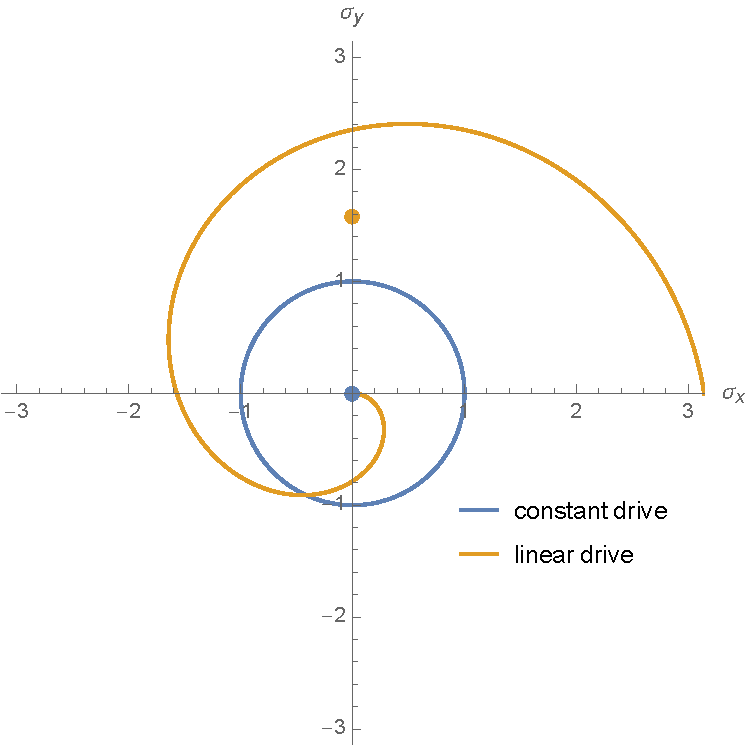
\includegraphics[width=0.5\textwidth]{figures/avg-CR-wave-rotation-lindrive.pdf}
	\caption{\textbf{Effect of the counter-rotating wave in the first order Magnus expansion.} The $\sx$ and $\sy$ projections of the counter-rotating wave contribution, $E(t) \left[\cos(2 \omega t) \sx + \sin(2 \omega t) \sy \right]$, are traced for $t \in [t_0,t_0+t_c]$ with $t_0=0$. Trajectories are shown both for constant drive $E(t) = 1$ and for a linearly increasing drive $E(t)=(t-t_0)$. The average projections are indicated with a dot. For constant drive, it can be seen that the average projection is zero, while for linear drive, the average is non-zero and directed $\pi/2$ radians from the initial (and final) projection. Choosing a different $t_0$ has the effect of rotating the trajectories and still leaves a non-zero average of equal magnitude in the linear drive case.}
	\label{fig:avg-crwave-rotation-lindrive}
\end{figure}

\subsubsection{Effective Hamiltonian}
Let's see if we can find an effective Hamiltonian that corresponds to (\ref{eq:evexp-order-1}). Per the procedure described in Daniel's notes, we proceed order by order of $1 / \omega$, such that $H_{eff}^{(m)}=\sum_{n=0}^m (1 / \omega)^n h_n$, where each $h_n$ may not depend explicitly on $t$ or $\omega$ and occurences of $t_0$ in (derivatives of) $H_1(t_0)$ are promoted to the instantaneous time $t$. We start with the trivial order $1 / \omega^0 = 1$. In this case, $h_0$ is given by 
\begin{align}
	h_0 = \left[\frac{E(t_0)}{4}\sx\right]_{t_0 \to t} = \frac{H(t)}{4}\sx. \label{eq:heff-order-0}
\end{align}
For the next order $1 / \omega^1$ we use the iterative relation 
\begin{align}
	h_{n+1} = C[\bar{H}(t_0), 1 / \omega, n+1] - C[\bar{H}_{eff}^{(n)}(t_0),1/\omega,n+1].
\end{align}
The first term is readily extracted from (\ref{eq:evexp-order-1}) and equal to
\begin{align}
	C[\bar{H}(t_0), 1 / \omega, 1] = \frac{E_1}{8 \omega} \left( \pi \sx + \sin(2 \omega t_0) \sx + \cos(2 \omega t_0) \sy \right).
\end{align}
The second term is obtained by calculating the Magnus expansion of (\ref{eq:heff-order-0}) up to first order in $1 / \omega$. Noting that $h_0$ is proportional to $\sx$ for all times and $[h_0(t_1),h_0(t_2)] = 0$ for all $t_1, t_2$, the first order Magnus expansion is exact and given by
\begin{align}
	\bar{H}_{eff}^{(0)}(t_0) = \left[ \frac{E(t_0)}{4} + \frac{E_1}{8 \omega} \pi \right] \sx.
\end{align}
Therefore,
\begin{align}
	C[\bar{H}_{eff}^{(0)}(t_0),1/\omega,1] = \frac{E_1}{8 \omega} \pi \sx,
\end{align}
leaving us with
\begin{align}
	h_1 = \frac{E_1}{8 \omega} \left( \sin(2 \omega t_0) \sx + \cos(2 \omega t_0) \sy \right).
\end{align}

Let's see if taking the Magnus expansion of this effective Hamiltonian indeed matches the ME of the real Hamiltonian over an interval $t_c$. As per the notebook `linear\_drive\_manual\_integration.nb' it does, up to first order! There is however a third order term (and higher order terms) that explains the deviation of the trajectory of the effective Hamiltonian from the stroboscopic evolution given by repeated application of $\exp[-i t_c \bar{H}(t_0 + k t_c)]$ with increasing $k$, as observed in numerical simulations for large driving strengths.

\subsection{Second order Magnus expansion}
We now continue by investigating the second order term in the Magnus expansion, given by (\ref{eq:omg-2}), to gain some intuition. We first focus on rewriting the commutator in the integrand:
\begin{alignat}{1}
	&\frac{1}{2}\big[ \tilde{H}(t_1), \tilde{H}(t_2) \big] = \frac{1}{2}\left[ -iH(t_1), -iH(t_2) \right] = - \frac{1}{2}\left[ H(t_1), H(t_2) \right] \nonumber \\
	&= -\frac{E(t_1)E(t_2)}{32} \big[ \left( (1 + \cos(2 \omega t_1)) \sx - \sin(2 \omega t_1) \sy \right), \left( (1 + \cos(2 \omega t_2)) \sx - \sin(2 \omega t_2) \sy \right) \big] \nonumber \\
	&= \frac{E(t_1)E(t_2)}{32} \Big( (1 + \cos(2 \omega t_1))\sin(2 \omega t_2) \left[  \sx, \sy \right] + \sin(2 \omega t_1) (1 + \cos(2 \omega t_2)) \left[\sy,\sx\right] \Big) \nonumber \\
	&= i \frac{E(t_1)E(t_2)}{32} \Big( (1 + \cos(2 \omega t_1))\sin(2 \omega t_2) - \sin(2 \omega t_1) (1 + \cos(2 \omega t_2)) \Big) \sz \label{eq:o2-itgd-expandedform} \\
	&= -i\frac{E(t_1)E(t_2)}{4} \cos(\omega t_1) \cos(\omega t_2) \sin(\omega(t_1 - t_2)) \sz \label{eq:o2-itgd-condensedform}.
\end{alignat}
A few important qualitative properties of the integrand and thus of the second order Magnus expansion term can be inferred from (\ref{eq:o2-itgd-condensedform}). Firstly, containing only the commutator $[\sx,\sy]$, the integrand is proportional to $\sz$ and represents the second order ``composition effect'' of non-commuting rotations around different axes in the $x-y$ plane. Furthermore, for $t_1 = t_2$ the final sine factor is zero, as is to be expected for the commutator at equal times.

% After plugging in the linear drive envelope, we arrive at the integrand
% \begin{align}
% 	-i\frac{(E_0 + E_1 t_1)(E_0 + E_1 t_2 )}{4} \cos(\omega t_1) \cos(\omega t_2) \sin(\omega(t_1 - t_2)) \sz.
% \end{align}
Noting that this integrand is to be doubly integrated over $t_1$ and $t_2$, it is wise to make the integrand separable into factors only depending on $t_1$ or $t_2$. This yields the integrand
\begin{alignat}{2}
	& &&\frac{-iE(t_1)E(t_2)}{4} \cos(\omega t_1) \cos(\omega t_2) \left( \sin(\omega t_1)\cos(\omega t_2) - \cos(\omega t_1)\sin(\omega t_2) \right) \sz \nonumber \\
	&= &&\frac{-i}{8} \sz \left( E(t_1) \sin(2 \omega t_1) E(t_2) \cos(\omega t_2)^2 \right) + \frac{i}{8} \sz \left( E(t_1) \cos(\omega t_1)^2 E(t_2) \sin(2 \omega t_2) \right). \label{eq:o2-itgd-separable}
\end{alignat}
We proceed by performing the inner integrals over $\mathrm{d}t_2$, resulting in
\begin{alignat}{2}
	&\int_{t_0}^{t_1} \mathrm{d}t_2\, E(t_2) \cos(\omega t_2)^2 &&= \int_{t_0}^{t_1} \mathrm{d}t_2\, (E_0 + E_1 t_2) \cos(\omega t_2)^2 \nonumber \\
	& &&= \frac{1}{4}(t_1 - t_0)\left( E(t_0) + E(t_1) \right) \nonumber \\
	& &&+ \frac{1}{4\omega} \left( E(t_1) \sin(2 t_1 \omega) - E(t_0) \sin(2 t_0 \omega) \right) \nonumber  \\
	& &&+ \frac{E_1}{8 \omega^2} \left( \cos(2 t_1 \omega) - \cos(2 t_0 \omega) \right) \label{eq:o2-itgd-inner1}\\
	&\int_{t_0}^{t_1} \mathrm{d}t_2\, E(t_2) \sin(2 \omega t_2) &&= \int_{t_0}^{t_1} \mathrm{d}t_2\, (E_0 + E_1 t_2) \sin(2 \omega t_2) \nonumber \\
	& &&= \frac{1}{2 \omega} \left( E(t_0) \cos(2 t_0 \omega) - E(t_1) \cos(2 t_1 \omega) \right) \nonumber \\
	& &&+ \frac{E_1}{4 \omega^2} \left( \sin(2 t_1 \omega) - \sin(2 t_0 \omega) \right). \label{eq:o2-itgd-inner2}
\end{alignat}
Plugging (\ref{eq:o2-itgd-inner1}) and (\ref{eq:o2-itgd-inner2}) into the integral of (\ref{eq:o2-itgd-separable}) over $\mathrm{d}t_2 \in [t_0,t_1]$ yields
\begin{alignat}{2}
	&-\frac{i}{8} \sz  E(t_1) \sin(2 \omega t_1) \Big( && \frac{1}{4}(t_1 - t_0)\left( E(t_0) + E(t_1) \right) \nonumber \\
	& &&+ \frac{1}{4\omega} \left( E(t_1) \sin(2 t_1 \omega) - E(t_0) \sin(2 t_0 \omega) \right) \nonumber  \\
	& &&+ \frac{E_1}{8 \omega^2} \left( \cos(2 t_1 \omega) - \cos(2 t_0 \omega) \right) \Big)  \nonumber \\
	&+ \frac{i}{8} \sz  E(t_1) \cos(\omega t_1)^2 \Big( &&\frac{1}{2 \omega} \left( E(t_0) \cos(2 t_0 \omega) - E(t_1) \cos(2 t_1 \omega) \right) \nonumber \\
	& &&+ \frac{E_1}{4 \omega^2} \left( \sin(2 t_1 \omega) - \sin(2 t_0 \omega) \right) \Big),
\end{alignat}
which thankfully can be simplified (by Mathematica, not by me...) to
\begin{align}
	&\frac{i}{16}\sz E(t_1)\cos(\omega t_1) (t_0-t_1)(E(t_0) + E(t_1))\sin(\omega t_1) \nonumber \\
	&-\frac{i}{16 \omega} \sz E(t_1)\cos(\omega t_1)(E(t_1)\cos(\omega t_1) -E(t_0) \cos(\omega(2 t_0 - t_1))) \nonumber \\
	&+\frac{i E_1}{32 \omega^2}\sz E(t_1) \cos(\omega t_1) (\sin(\omega t_1) - \sin(\omega (2 t_0-t_1))).
\end{align}
Finally, we calculate the second order Magnus exponent term by integrating the previous expression with respect to $\mathrm{d}t_1$ over an evolution interval $t_c$, starting from $t_0$:
\begin{align}
	\frac{i}{t_c}\Omega_2(t_0+t_c,t_0) &= \frac{E(t_0)^2}{32 \omega} \sz (1 - 2 \cos(2 \omega t_0)) \nonumber \\
	&+\frac{E_1 E(t_0)}{32 \omega^2} \sz \left( \pi - 2\pi \cos(2 \omega t_0) - 3 \sin(2 \omega t_0)\right) \nonumber \\
	&+\frac{E_1^2}{384 \omega^3} \sz \left( 3 + 4\pi^2 + (18 - 6 \pi^2) \cos(2 \omega t_0) + 18\pi\sin(2 \omega t_0)\right) \label{eq:o2-term}.
\end{align}
Direct calculation of the second order Magnus term using Daniel's scripts yields the same expression, which is comforting.

The first term of (\ref{eq:o2-term}) represents the Bloch-Siegert shift and is the only term that survives for a constant drive with $E_1 = 0$. For $t_0 = k t_c$, we can understand the second term and the parts of third term that contain $\pi^2$ as the increase in Bloch-Siegert shift during the evolution interval $t_c$, similar to (\ref{eq:evexp-rwa-linear-term}).

Noting that the expressions and integrals become increasingly complicated for higher order Magnus terms, we stop here with the manual integration and intuitive interpretation of the Magnus terms.

\section{Impulse operators}
The effective Hamiltonian generated from the Magnus expansion is applicable if the driving envelope is varied analytically. However, if the driving envelope experiences a non-analytical change, such as a sudden turn-on, an extra ``impulse operator'' is needed to describe the ``jump'' between the effective trajectory before and after the change. In this section we will work towards the development of such impulse operators.

\subsection{Constant drive}
Constant drive\todo{summarize findings for constant drive}

\subsection{Linear drive}

% \begin{alignat}{3}
% 	&\Omega_2(t,t_0) &&= \phantom{-} \frac{1}{2}\int_{t_0}^t \mathrm{d}t_1 \int_{t_0}^{t_1} \mathrm{d}t_2 \big[ && -iH(t_1), -iH(t_2) \big] \nonumber \\
% 	& &&= - \frac{1}{2}\int_{t_0}^t \mathrm{d}t_1 \int_{t_0}^{t_1} \mathrm{d}t_2 \big[ &&\frac{E(t_1)}{4}\left( (1 + \cos(2 \omega t_1)) \sx - \sin(2 \omega t_1) \sy \right), \nonumber \\ 
% 	& && &&\frac{E(t_2)}{4}\left( (1 + \cos(2 \omega t_2)) \sx - \sin(2 \omega t_2) \sy \right) \big]
% \end{alignat}

\printbibliography
	
\end{document}